Voici quelques exemples de modèles SimplePDL (sans ressources) :

\begin{figure}[h]
   \centering
   \subfloat[Processus simple]{\label{process_simple_pdl}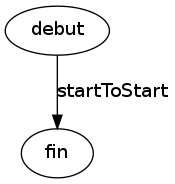
\includegraphics[width=0.18\textwidth]{../Images/model_process_simple_pdl.png}}
   \subfloat[Processus]{\label{process_pdl}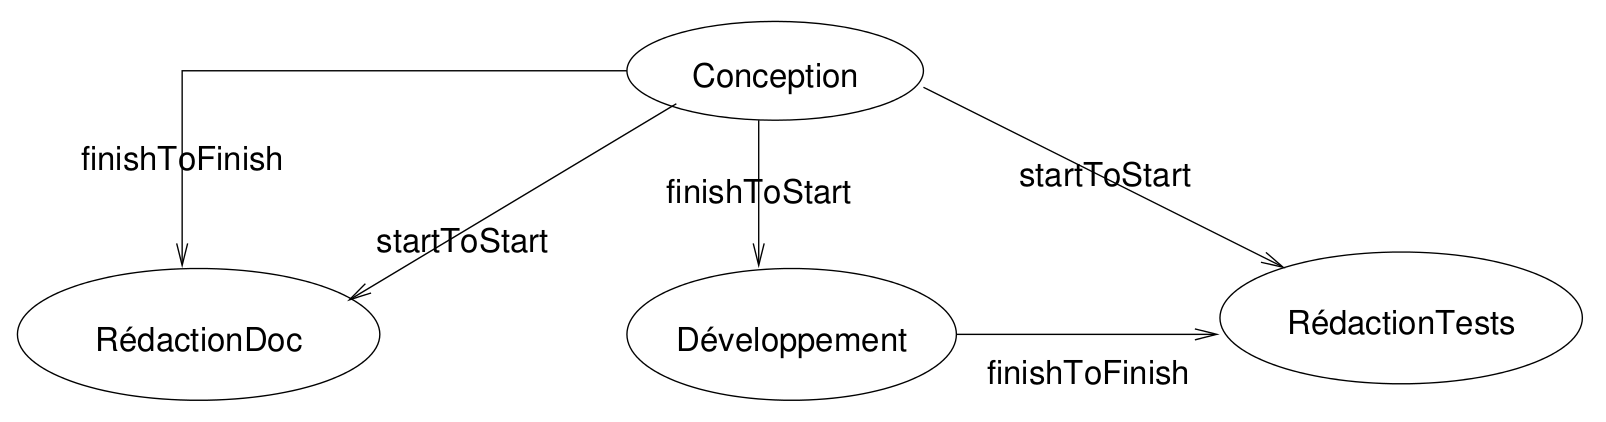
\includegraphics[width=0.7\textwidth]{../Images/model_process_pdl.png}}
   \caption{Exemples de modèles de processus SimplePDL}
\end{figure}

\vspace{1em}
Et quelques exemples de modèles PetriNet :
\begin{figure}[h]
   \centering
   \subfloat[Exemple]{\label{exemple_net}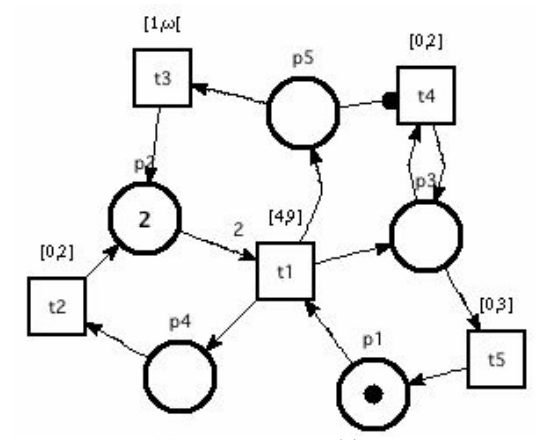
\includegraphics[width=0.5\textwidth]{../Images/model_exemple_net.png}}
   \subfloat[4 saisons]{\label{saisons_net}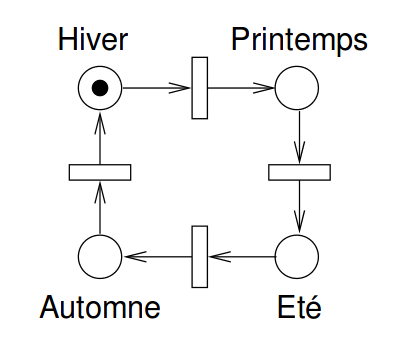
\includegraphics[width=0.5\textwidth]{../Images/model_saisons_net.png}}
   \caption{Exemples de modèles de réseaux de pétri}
\end{figure}
